\chapter{Wstęp}
\label{cha:Wstęp}

Celem projektu jest wykonanie i przetestowanie nowego interfejsu człowiek-maszyna, który wykorzysta jeden z dostępnych algorytmów rozpoznawania języka naturalnego.

We współczesnym świecie można znaleźć wiele przykładów sterowania maszynami. Jedną z nich jest między innymi łazik planetarny Kalman, projekt rozwijany przez członków koła naukowego AGH Space Systems.  Sterowanie poruszaniem się tego robota możliwe jest poprzez wykorzystanie skonstruowanego przez studentów urządzenia \cite{jklazik}. Za pomocą odpowiednich przycisków i gałek uruchamiane są odpowiadające im części napędu jezdnego. Innowacyjna konstrukcja tego urządzenia i modernizacja sposobu sterowania robotem, który z naciskania przycisków na klawiaturze laptopa przerodził się w osobny moduł jedynie podłączany kablem nasuwa sugestię możliwości pójścia o krok dalej.

Co gdyby algorytm sterowania maszyną został przeniesiony z powrotem do komputera, ale pozbawiony potrzeby wchodzenia w kontakt fizyczny poprzez umożliwienie sterowania głosowego? Jest to pytanie na które odpowiedź jest stawiana w wielu dziedzinach życia codziennego, zaczynając od asystentów obecnych w każdym smartfonie, poprzez obsługiwanie funkcji w samochodach, a kończąc na aktywacji urządzeń przemysłowych. Jest to nie tylko funkcjonalność przydatna w momencie, kiedy osoba obsługująca daną maszynę nie ma możliwości wykonania danej czynności własnoręcznie. Dla osób niepełnosprawnych, posiadających ograniczenia ruchowe, jest to niejednokrotnie umożliwienie używania danego urządzenia i poszerzenie zakresu dostępności.

Jak wiele nowatorskich dziedzin rozwoju, również i ta technologia wymaga pracy nad nią i ciągłego dostosowywania jej do codziennych potrzeb. Biorąc na przykład asystenta głosowego Google, dostępnego w większości telefonów komórkowych z Androidem, już po krótkim czasie używania można zauważyć występujące czasem nieścisłości w rozpoznawaniu i rozumieniu przez aplikację danej wypowiedzi. Jest to bezpośrednio powiązane z zastosowanymi algorytmami rozpoznawania głosowego, które inaczej niż człowiek, nie zawsze są w stanie poprawnie zinterpretować ludzką mowę. 

Praca dyplomowa obejmie przegląd istniejących możliwości sterowania głosowego urządzeniami. Zaprezentowana zostanie analiza wykorzystywanych w prototypowych aplikacjach modeli uczenia maszynowego, a na jej podstawie napisany algorytm służący do sterowania głosowego. Poprawność implementacji zweryfikuje podłączenie algorytmu w środowisku Robot Operating System do symulacji przykładowego robota w programie Gazebo. Następnie przy użyciu biblioteki Custom Tkinter zostanie wykonany interfejs służący do sterowania robotem.


%---------------------------------------------------------------------------

\section{Rozpoznawanie głosowe}
\label{sec:rozpoznawanieGlosowe}

Rozpoznawanie głosu to umiejętność wykonywania przez urządzenie identyfikacji zadanych mu komend. Dzieje się to poprzez wykorzystanie konwersji A/D do przetworzenia sygnału analogowego w cyfrowy (Rys.\ref{fig:ad}). 

\begin{figure}[h]
    \centering
    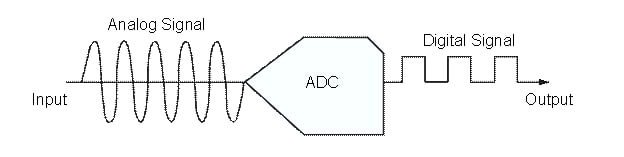
\includegraphics[width=0.95\linewidth]{files/ad.jpg}
    \caption{Konwersja A/D. (Źródło: \url{https://wiki.analog.com/university/courses/electronics/text/chapter-20})}
    \label{fig:ad}
\end{figure}

Komputer do rozszyfrowania sygnału cyfrowego, musi posiadać bazę słów i sylab do porównywania ich do siebie. W rzeczywistości, aby algorytm służący do rozpoznawania głosu był w stanie poprawnie przetworzyć zadaną mu komendę, potrzebuje sporej ilości pamięci RAM, aby wystarczająco szybko znaleźć odpowiadający sygnałowi cyfrowemu wzorzec. Analizowana jest nie tylko sama treść, ale również częstotliwość głosu, akcent czy poprawność wymowy. Ponadto, sygnał analogowy musi zostać wcześniej przeprocesowany, celem pozbycia się szumów lub dźwięku w tle.

Technologie służące rozpoznawaniu głosu przebyły długą drogę aby znaleźć się we współczesności. Idea stworzenia urządzenia, które jest w stanie rozpoznawać mowę i przetwarzać ją na tekst narodziła się z prostej ludzkiej chęci to usprawniania powtarzających się zadań. Już w XIX wieku powstało pierwsze urządzenie rejestrujące dźwięk, które niedługo później przerodziło się w znany nam obecnie dyktafon, a zapoczątkowało falę mechanizacji pracy biurowej. Wprowadzone w życie codzienne zostały między innymi maszyny do pisania, które swoją przydatnością wpłynęły na wytworzenie się konceptu aktywowanej głosowo maszyny do pisania. 

Próby wytworzenia urządzenia zdolnego do automatycznego rozpoznawania głosu były w większości oparte na podstawowych elementach fonetycznych języka i tego jaki jest proces ich tworzenia. Aby wyprodukować dźwięk samogłoski, struny głosowe muszą odpowiednio wibrować, aby powietrze które przepływa przez nie uzyskało odpowiednią częstotliwość. Fakt ten został wykorzystany w 1952 roku, kiedy to Davis, Biddulph, i Balashek z Bell Laboratories stworzyli pierwszy system do rozpoznawania głosowego, zdolny do interpretacji cyfr mówionych przez jednego z twórców. Na podstawie wartości pasm częstotliwości dźwięku każdej samogłoski powstał wzór dla maszyny, z którego mogła ona odczytać region występowania częstotliwości dla każdej z cyfr. Następnie odnosząc się do posiadanego wzoru mogła ona zidentyfikować daną cyfrę \cite{juang2005automatic}.

Współczesne urządzenia posiadające funkcję rozpoznawania głosowego zawierają w sobie nie tylko odpowiednie elementy mechaniczne i elektroniczne. Na możliwość wykonywania tej czynności składają się algorytmy uczenia maszynowego i sieci neuronowe. Z najbardziej rozpoznawalnych i ogólnie dostępnych na rynku zastosowań można wyróżnić między innymi elementy \textit{smart home} takie jak Apple HomeKit, Amazon Alexa czy dostępny w wielu smartfonach Google Assistant.


%---------------------------------------------------------------------------

\section{Przetwarzanie języka naturalnego}
\label{sec:przetwarzanieJezykaNaturalnego}

Natural Language Processing (NLP) jest to dziedzina sztucznej inteligencji zajmująca się szeroko pojętą komunikacją pomiędzy człowiekiem a maszyną. Jednym ze sposobów, w jaki można skategoryzować język, służący do takiej właśnie komunikacji, jest podział na \textit{naturalny} oraz \textit{nienaturalny}. Część naturalna odnosi się do wymiany informacji pomiędzy człowiekiem a robotem w sposób najbardziej zbliżony do komunikacji pomiędzy ludźmi, za pomocą słów złożonych w zdania o zadanym kontekście. Język \textit{nienaturalny} natomiast opisuje obszar komunikacji, w którym można zawrzeć między innymi języki programowania czy funkcjonalności pozwalające na obsługę maszyn w sposób dla nich domyślny, który od człowieka wymaga wcześniejszego doświadczenia. 

Język \textit{naturalny} podzielić można na dwie kategorie komunikacji: niewerbalną i werbalną. Pierwsza z nich obejmuje każdy przekaz, jaki człowiek może nadać, nie używając do wykonania tej czynności języka mówionego. Może być to ton głosu, postawa, gestykulacja, mimika twarzy, ale również dystans między rozmówcami, styl ubioru czy czas oraz miejsce konwersacji. Komunikacja niewerbalna niejednokrotnie niesie za sobą znaczenie przekazu, na które odbiorca może zareagować w określony dla danej sytuacji sposób. 

Komunikację werbalną, która opiera się na języku mówionym, w przetwarzaniu języka naturalnego można zobrazować jako widoczny na Rys.\ref{fig:nlp} proces przetwarzania dźwięku wydanego przez człowieka na wyrazy, a następnego ekstrakcję znaczenia i informacji z przekazu.

\begin{center}
    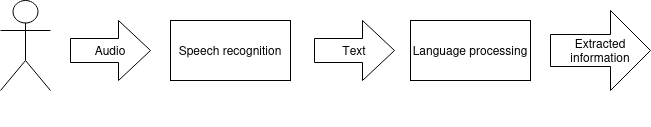
\includegraphics[width=0.95\linewidth]{files/nlp.png}
    \captionof{figure}{Przetwarzanie języka naturalnego.}
    \label{fig:nlp}
\end{center}

%---------------------------------------------------------------------------

\subsection{Symboliczne przetwarzanie języka naturalnego}
\label{subsec:symbolic}

Do procesu przetwarzania języka naturalnego można podejść na wiele sposobów. Głównymi rozwiązaniami są systemy oparte na zestawie reguł i zasad (Symbolic NLP), oparte na prawdopodobieństwie (Statistical NLP) i oparte na sieciach neuronowych (Neural NLP). Pierwsze z nich do poprawnego działania wymagają stworzonej manualnie, obszernej bazy wiedzy, wykorzystywanej do ekstrakcji informacji, rozpoznawania konkretnych wzorców czy przeprowadzania klasyfikacji tekstu. 

Z uwagi na fakt, że język mówiony ciągle się zmienia, tj. tworzone są nowe zasady, formy gramatyczne oraz słowa, aby nadążyć za rozwojem ludzkości, implementacja wszystkich rządzących nim praw jest uciążliwa i czasochłonna. W związku z tym, systemy te często poza konkretnymi regułami, opierają się również na wykluczeniu niewystępujących naturalnie scenariuszy konwersacji. Bazując na tym systemie, proces przetwarzania przebiega następująco (Rys. \ref{fig:symbolic}): na podstawie charakterystyki danego zadania, tworzone są reguły spełniające założenia. Reguły te są iteracyjnie nakładane na dane wejściowe celem znalezienia istniejących wzorców i procesowane zgodnie z otrzymanymi rezultatami aby zwiększyć dokładność algorytmu. 

\begin{center}
    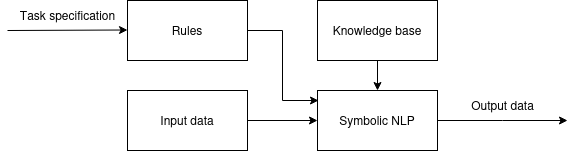
\includegraphics[width=0.95\linewidth]{files/symbolic.png}
    \captionof{figure}{Symboliczne przetwarzanie języka naturalnego.}
    \label{fig:symbolic}
\end{center}

Pomimo tego, że systemy oparte na zestawie reguł i zasad są dokładne i rzetelne, jeśli zaimplementowane prawidłowo, aby były efektywne mogą być głównie stosowane do wykonywania mało złożonych zadań, ściśle określonych i z nałożonymi ograniczeniami. 

%---------------------------------------------------------------------------

\subsection{Statystyczne przetwarzanie języka naturalnego}
\label{subsec:statistyc}

W przypadku, gdy dane zadanie posiada wiele złożonych scenariuszy, stosowane są systemy oparte na prawdopodobieństwie, gdzie algorytm uczy się własnego działania na podstawie podanych mu wcześniej danych. Uczenie może przebiegać na jeden z trzech sposobów: 
\begin{itemize}
    \item uczenie nadzorowane (ang. supervised learning), gdzie model dostaje dane wejściowe oraz pożądane dane wyjściowe, a jego zadaniem jest znalezienie ścieżki pomiędzy nimi,
    \item uczenie nienadzorowane (ang. unsupervised learning), gdzie bazując tylko na danych wejściowych, model ma za zadanie wyciągnąć z nich informacje, 
    \item uczenie przez wzmacnianie (ang. reinforcement learning), gdzie zamiast podania modelowi danych, jest on umieszczany w środowisku, w którym poprzez automatyczne wyciąganie danych ma osiągnąć zadany cel. 
\end{itemize}

Na osiągnięte przez model rezultaty, wpływa nie tylko jakość danych, ale również sposób, w jaki informacje z nich są wyciągane. Podając algorytmowi do przetworzenia przykładowe zdanie, do wyciągnięcia informacji może on użyć \textit{kodowania 1 z n} (Rys. \ref{fig:one-hot}), gdzie w wektorze n-wymiarowym każdy element może mieć wartość 1 lub 0 w zależności czy w zdaniu o długości n występuje słowo istniejące w słowniku, czy nie. Do podejścia tego, można dołożyć częstość występowania słów, gdzie w wektorze odnoszącym się do danego słowa, zamiast 1 podana będzie jego liczność. 

\begin{center}
    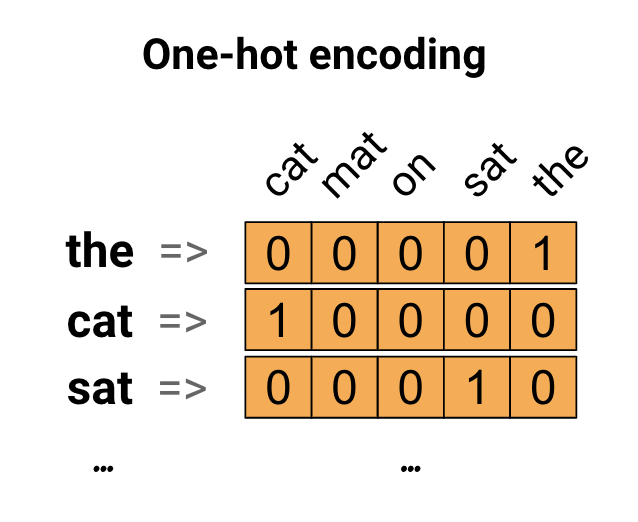
\includegraphics[width=0.6\linewidth]{files/one-hot.png}
    \captionof{figure}{Kodowanie 1 z n. (Źródło: \url{https://www.tensorflow.org/text/guide/word_embeddings})}
    \label{fig:one-hot}
\end{center}

Nie tylko ze zdań można wyciągać informacje służące do przewidywania kolejnych elementów, ale również znaków czy sekwencji słów. Używając modeli \textit{n-gram}, które tworzą wektor wystąpień nie pojedynczego słowa, ale dwóch (bigrams) lub trzech (trigrams) (Rys.\ref{fig:n-gram}), można znacznie zwiększyć skuteczność modelu, ponieważ bierze on pod uwagę kontekst występowania słów w sekwencji. 

\begin{center}
    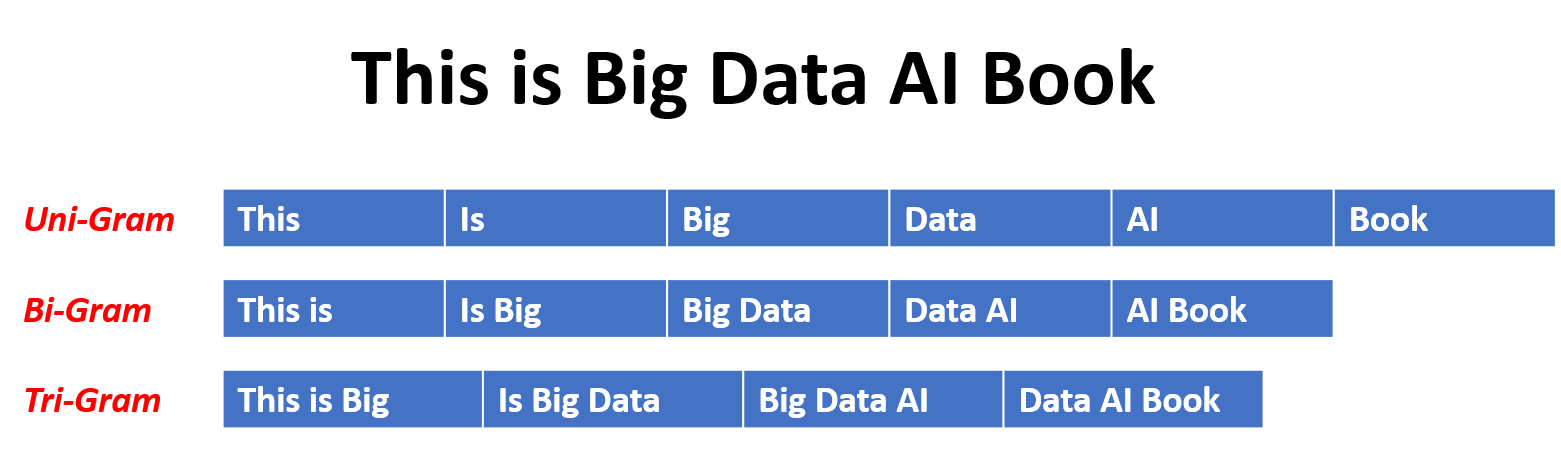
\includegraphics[width=0.8\linewidth]{files/n-grams.png}
    \captionof{figure}{Unigram, bigram i trigram. (Źródło: \url{https://devopedia.org/n-gram-model#Mehmood-2019})}
    \label{fig:n-gram}
\end{center}

%---------------------------------------------------------------------------

\subsection{Neuronowe przetwarzanie języka naturalnego}
\label{subsec:neural}

Pomimo swojej szeroko pojętej użyteczności i zastosowań, nie wszystkie złożone problemy mogą zostać objęte podejściem statystycznym. Do wyciągnięcia niskopoziomowych właściwości tekstu czy radzenia sobie z długimi i skomplikowanymi danymi wejściowymi implementowane są sieci neuronowe. 

Używając uczenia nadzorowanego, wektory zawierające cechy każdego ze słów w danych wejściowych używane są do nauczenia modelu przewidywania następnych słów w podanym kontekście. Pojedyncze wykonanie tej czynności to \textit{warstwa} przez którą przechodzą dane w modelu. Warstwy te, nakładane na siebie tworzą właśnie sieci neuronowe. 

Współczesne systemy do rozpoznawania głosu bazują na ukrytym modelu Markova (hidden Markov model). Model ten opisuje obserwowalny proces (Rys. \ref{fig:markov}) A, którego rezultat zależy od rezultatu procesu E. Ponieważ stan E nie jest obserwowalny, jego stan może być znaleziony poprzez obserwację stanu A. Jest to adekwatne przedstawienie tego, czym jest proces występowania każdego po sobie wyrazu w zdaniu. Na podstawie ciągu składającego się ze znanego słowa i kolejnego, które wystąpi po nim, możliwe jest statystyczne przybliżenie wartości słowa nieznanego. Następnie w tym procesie sieci neuronowe rekurencyjnie używają danych wyjściowych z modelu dla poprzedniego kroku do wpłynięcia na dane wejściowe do kolejnego w sekwencji. 

\begin{center}
    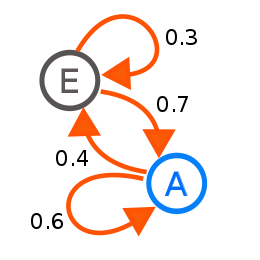
\includegraphics[width=0.5\linewidth]{files/markov.png}
    \captionof{figure}{Diagram przedstawiający proces Markova. (Źródło: \url{https://commons.wikimedia.org/wiki/File:Markovkate_01.svg})}
    \label{fig:markov}
\end{center}

%---------------------------------------------------------------------------
